\documentclass{article}
\setlength{\parindent}{0pt}
\setlength{\parskip}{1em}
\setlength{\columnsep}{3cm}

\usepackage{xcolor}
\usepackage{multicol}
\usepackage{unicode-math}
\usepackage{listings}
\usepackage{lualatex-math}
\setmainfont[
  BoldFont={STIXTwoText-Bold},
  ItalicFont={STIXTwoText-Italic},
  BoldItalicFont={STIXTwoText-BoldItalic}
]{STIXTwoText-Regular}
\setmathfont{STIXTwoMath-Regular}

\usepackage{biblatex}
\addbibresource{references.bib}

\usepackage{tikz}
\usetikzlibrary{automata, trees, positioning, arrows, fit, matrix, shapes.geometric, shapes.misc, calc}
\pgfdeclarelayer{background}
\pgfdeclarelayer{foreground}
\pgfsetlayers{background,main,foreground}

\newcommand\Var[1]{\textcolor{blue}{#1}}
\newcommand\Num[1]{\textcolor{orange}{#1}}
\newcommand\Keyword[1]{{\textbf{\texttt{#1}}}}
\newcommand\Fun[1]{{\texttt{#1}}}

\lstnewenvironment{CITY}[1][]
{
    \lstset{
        mathescape=true,
        basicstyle=\footnotesize, 
        basicstyle=\ttfamily,
        stringstyle=\color{teal},
        morestring=[b]",
        showstringspaces=false,
        keywords={,let,if,else,in,city,road,building,for,foreach,to,procedure,lambda,park,field,tree,junction,river,lake,restaurant, nil,},
        escapeinside={@}{@},
        xleftmargin=.04\textwidth,
        #1
    }
}
{}

\title{Projektna naloga}
\author{PPJ}

\begin{document}
\maketitle

Cilj projektne naloge je izdelava domensko specifičnega jezika za opis infrastrukture v mestu.
Za dokončanje projekta so potrebni naslednji koraki:

\begin{enumerate}
\item Zasnova jezika, določitev konstruktov in sintakse jezika
\item Priprava smislenih testnih primerov
\item Definicija sintakse z gramatiko in regularnimi izrazi
\item Implementacija abstraktnega sintaktičnega drevesa
\item Konstrukcija končnega avtomata
\item Implementacija pregledovalnika (\emph{scannerja})
\item Izračun \textsc{FIRST} in \textsc{FOLLOW} množic
\item Implementacija razčelenejvalnika (\emph{parserja})
\item Implementacija pretvorbe v niz (\emph{minifier} ali \emph{pretty-printer})
\item Implementacija izvoza v GeoJSON
\end{enumerate}

\textbf{Jezik morate zasnovati sami, torej sami določite konstrukte in sintakso jezika.}

Jezik opisan v tem dokumentu naj služi predvsem za inspiracijo.

\newpage
\section{Osnova}
Zahtevano je, da lahko z uporabo vašega jezika opišete vsaj zgradbe in ceste v mestu.
Torej je potrebno podpreti polilinije (\emph{polyline}) in poligone (\emph{polygon}).
Na primer, majhen del mesta bi lahko opisali takole:

\begin{multicols}{2}
\begin{CITY}
  city "Fiesa" {
    road "Oljcna pot" {
      bend((@\Num{1}@, @\Num{1}@), (@\Num{2}@, @\Num{2}@), @\Num{20}@);
      bend((@\Num{2}@, @\Num{2}@), (@\Num{3}@, @\Num{1}@), @\Num{40}@);
      line((@\Num{2}@, @\Num{2}@), (@\Num{2}@, @\Num{5}@));
      bend((@\Num{2}@, @\Num{3}@), (@\Num{5}@, @\Num{4}@), @\Num{20}@);
      line((@\Num{5}@, @\Num{4}@), (@\Num{6}@, @\Num{4}@))
    };
    building "Soncne terase" {
      box((@\Num{3}@, @\Num{2}@), (@\Num{5}@, @\Num{3}@))
    };
    building "Dom Fiesa" {
      box((@\Num{0.5}@, @\Num{3.5}@), (@\Num{1.5}@, @\Num{2.5}@))
    };
    building "LaRocca" {
      box((@\Num{0.5}@, @\Num{5}@), (@\Num{1.5}@, @\Num{4}@))
    };
    building "Hotel Fiesa" {
      box((@\Num{1.75}@, @\Num{1.5}@), (@\Num{2.25}@, @\Num{1}@))
    }
  }
\end{CITY}

\columnbreak

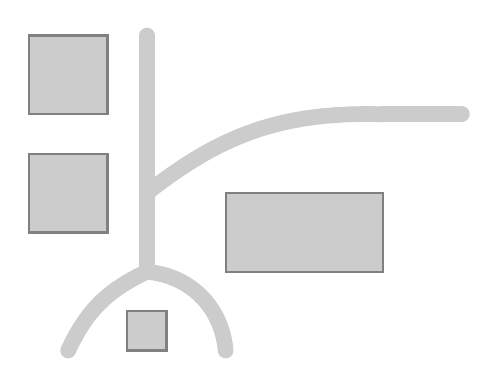
\begin{tikzpicture}
  \draw [line width=2mm, color=white!60!gray, line cap=round] (1, 1) to[bend left=20] (2, 2);
  \draw [line width=2mm, color=white!60!gray, line cap=round]  (2, 2) to[bend left=40] (3, 1);
  \draw [line width=2mm, color=white!60!gray, line cap=round]  (2, 2) to (2, 5);
  \draw [line width=2mm, color=white!60!gray, line cap=round]  (2, 3) to[bend left=20] (5, 4);
  \draw [line width=2mm, color=white!60!gray, line cap=round]  (5, 4) to (6, 4);

  \fill [thick, fill=white!60!gray, draw=gray] (3, 2) rectangle (5, 3);
  \fill [thick, fill=white!60!gray, draw=gray] (0.5, 3.5) rectangle (1.5, 2.5);
  \fill [thick, fill=white!60!gray, draw=gray] (0.5, 5) rectangle (1.5, 4);
  \fill [thick, fill=white!60!gray, draw=gray] (1.75, 1.5) rectangle (2.25, 1);
\end{tikzpicture}
\end{multicols}


\subsection{Konstrukti}
Uporabljen jezik vsebuje naslednje konstrukte.

\subsubsection{Enota}
Enota služi kot nevtralen element (NO-OP).
\begin{CITY}
  nil
\end{CITY}

\subsubsection{Realna števila}
\begin{CITY}
  @\Num{1}@
  @\Num{1.2}@
\end{CITY}

\subsubsection{Nizi}
\begin{CITY}
  "NIZ"
\end{CITY}

\subsubsection{Koordinate}
S koordinatami lahko predstavimo lokacije na zemljevidu, v tem primeru je prva komponenta longituda, druga komponenta pa je latituda.
\begin{CITY}
  (@\Var{X}@, @\Var{Y}@)
\end{CITY}

\subsubsection{Bloki}
Blok \Keyword{city} predstavlja mesto, ki ga opisujemo.
Vsebuje lahko bloke za opis cest in zgradb.
To je glaven element v jeziku.
\begin{CITY}
  city "NAME" {
    @\Var{BLOCKS}@
  }
\end{CITY}

Blok \Keyword{road} predstavlja cesto.
Vsebuje lahko ukaze za izris, ki izrišejo črte.
\begin{CITY}
  road "NAME" {
    @\Var{COMMANDS}@
  }
\end{CITY}

Blok \Keyword{builing} predstavlja zgradbo.
Vsebuje lahko ukaze za izris, ki izrišejo obrobo zapolnjenega lika.
Obroba lika mora biti zaključena, torej končna lokacija mora biti enaka prvi.
\begin{CITY}
  building "NAME" {
    @\Var{COMMANDS}@
  }
\end{CITY}

\subsubsection{Ukazi}

Bloka \Keyword{road} in \Keyword{building} lahko vsebujeta naslednje ukaze za izris.

Ukaz \Fun{line} izriše črto, med podanima lokacijama.
\begin{CITY}
  line(@\Var{POINT}@, @\Var{POINT}@)
\end{CITY}

Ukaz \Fun{bend} izriše krivuljo, med podanima lokacijama.
Podani kot določa stopnjo ukrivljenosti.
Če je kot $0^\circ$ se izriše ravna črta, če je kot $45^\circ$ se izriše približek četrtine krožnice.
Pozitivni koti pomenijo, da je krivulja nagnjena v levo, negativni koti pa pomenijo, da je krivulja nagnjena v desno.

\begin{CITY}
  bend(@\Var{POINT}@, @\Var{POINT}@, @\Var{ANGLE}@)
\end{CITY}

Ukaz \Fun{box} izriše pravokotnik, med podanima lokacijama.
Torej prva lokacija je zgornji levi kot pravokotnika, druga lokacija pa je spodnji desni kot.
\begin{CITY}
  box(@\Var{POINT}@, @\Var{POINT}@)
\end{CITY}

Ukaz \Fun{circ} izriše krog z izbranim polmerom na podani lokaciji.
Ta lokacija predstavlja center kroga.
\begin{CITY}
  circ(@\Var{POINT}@, @\Var{RADIUS}@)
\end{CITY}

\section{Nadgradnja}
Jezik nadgradite s poljubnimi konstrukti in funkcionalnostmi, ki so smiselne za vaš projekt.

V nadaljevanju sledi nekaj idej.

\subsection{Validacija}
Preverite smiselnost modela in uporabnika jezika opozorite na morebitne težave.
Za pohitritev iskanja presečišč lahko uporabite R-drevo (dovoljena je uporaba knjižnice).
Uporabite pa lahko tudi kateri koli drug temu namenjen algoritem iz računalniške geometrije.

\newpage

\subsubsection{Presečišča med poligoni}
Z jezikom je mogoče opisati presekajoče poligone, prav tako pa lahko imajo poligoni presečišča tudi samim s sabo.
V primeru, da ti predstavljajo zgradbe takšni poligoni niso smiselni.
Prav tako bomo imeli težave pri izrisu.
Zato lahko takšna presečišča najdemo in uporabnika nanj opozorimo.

\begin{multicols}{2}
\begin{CITY}
  city "Shapes" {
    building "Simple" {
      line((@\Num{0}@, @\Num{0}@), (@\Num{0}@, @\Num{2}@));
      line((@\Num{0}@, @\Num{2}@), (@\Num{2}@, @\Num{2}@));
      line((@\Num{2}@, @\Num{2}@), (@\Num{2}@, @\Num{0}@));
      line((@\Num{2}@, @\Num{0}@), (@\Num{0}@, @\Num{0}@))
    };
    building "Complex" {
      line((@\Num{3}@, @\Num{0}@), (@\Num{3}@, @\Num{2}@));
      line((@\Num{3}@, @\Num{2}@), (@\Num{5}@, @\Num{0}@));
      line((@\Num{5}@, @\Num{0}@), (@\Num{5}@, @\Num{2}@));
      line((@\Num{5}@, @\Num{2}@), (@\Num{3}@, @\Num{0}@))
    };
  }
\end{CITY}

\columnbreak

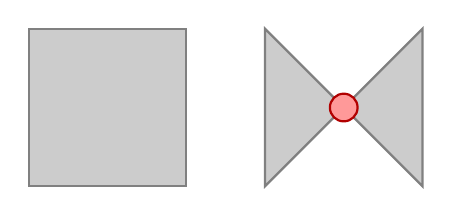
\begin{tikzpicture}
  \filldraw [thick, fill=white!60!gray, draw=gray] (0, 0) -- (0, 2) -- (2, 2) -- (2, 0) -- cycle;

  \filldraw [thick, fill=white!60!gray, draw=gray] (3, 0) -- (3, 2) -- (4, 1) -- cycle;
  \filldraw [thick, fill=white!60!gray, draw=gray] (4, 1) -- (5, 2) -- (5, 0) -- cycle;

  \filldraw[thick, fill=white!60!red, draw=black!30!red] (4, 1) circle (5pt);
\end{tikzpicture}
\end{multicols}

\subsubsection{Presečišča med polilinijami}
Pri polilinijah je manj težav, saj v primeru presečišč najverjetneje gre za nadvoz.
Kljub temu lahko uporabimo podobno kodo kot za presečišča med poligoni in uporabnika nanj opozorimo.

\begin{multicols}{2}
\begin{CITY}
  city "Shapes" {
    road "Simple" {
      line((@\Num{0}@, @\Num{0}@), (@\Num{0}@, @\Num{2}@));
      line((@\Num{0}@, @\Num{2}@), (@\Num{2}@, @\Num{2}@));
      line((@\Num{2}@, @\Num{2}@), (@\Num{2}@, @\Num{0}@));
      line((@\Num{2}@, @\Num{0}@), (@\Num{0}@, @\Num{0}@))
    };
    road "Complex" {
      line((@\Num{3}@, @\Num{0}@), (@\Num{3}@, @\Num{2}@));
      line((@\Num{3}@, @\Num{2}@), (@\Num{5}@, @\Num{0}@));
      line((@\Num{5}@, @\Num{0}@), (@\Num{5}@, @\Num{2}@));
      line((@\Num{5}@, @\Num{2}@), (@\Num{3}@, @\Num{0}@))
    };
  }
\end{CITY}

\columnbreak


\begin{tikzpicture}
  \draw [line width=2mm, color=white!60!gray, line cap=round] (0, 0) to (0, 2);
  \draw [line width=2mm, color=white!60!gray, line cap=round] (0, 2) to (2, 2);
  \draw [line width=2mm, color=white!60!gray, line cap=round] (2, 2) to (2, 0);
  \draw [line width=2mm, color=white!60!gray, line cap=round]  (2, 0) to (0, 0);

  \draw [line width=2mm, color=white!60!gray, line cap=round] (3, 0) to (3, 2);
  \draw [line width=2mm, color=white!60!gray, line cap=round] (3, 2) to (5, 0);
  \draw [line width=2mm, color=white!60!gray, line cap=round] (5, 0) to (5, 2);
  \draw [line width=2mm, color=white!60!gray, line cap=round] (5, 2) to (3, 0);

  \filldraw[thick, fill=white!60!blue, draw=black!30!blue] (4, 1) circle (5pt);
\end{tikzpicture}
\end{multicols}

\subsubsection{Presečišča med poligoni in polilinijami}
Prav tako lahko najdemo presešišča med poligoni in polilinijami.
Najverjetne gre tukaj za napako.
Sicer v redkih primerih se res lahko zgodi, da cesta gre skozi zgradbo, na primer pri bencinskih črpalkah.

\begin{multicols}{2}
\begin{CITY}
  city "Shapes" {
    road "Intersects" {
      line((@\Num{0}@, @\Num{0}@), (@\Num{6}@, @\Num{3}@))
    };
    building "Building" {
      box((@\Num{1}@, @\Num{1}@), (@\Num{5}@, @\Num{5}@))
    }
  }
\end{CITY}

\columnbreak

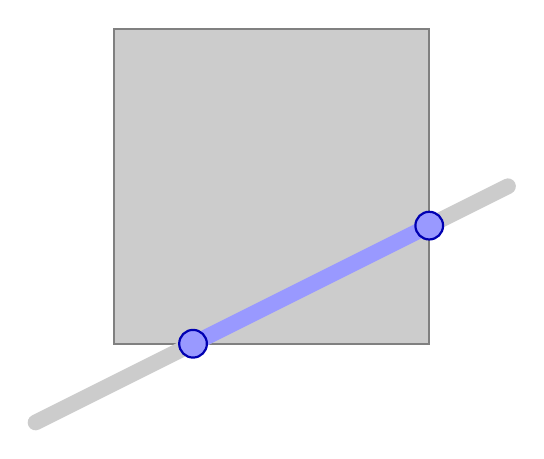
\begin{tikzpicture}
  \fill [thick, fill=white!60!gray, draw=gray] (1, 1) rectangle (5, 5);

  \draw [line width=2mm, color=white!60!gray, line cap=round] (0, 0) to (6, 3);
  \draw [line width=2mm, color=white!60!blue] (2, 1) to (5, 2.5);

  \filldraw[thick, fill=white!60!blue, draw=black!30!blue] (2, 1) circle (5pt);
  \filldraw[thick, fill=white!60!blue, draw=black!30!blue] (5, 2.5) circle (5pt);
\end{tikzpicture}
\end{multicols}


\subsubsection{Dotikališča med polilinijami}
Dotikališča polilinij označujejo križišča.
Uporabnika lahko opozorimo na njihove lokacije.

\begin{multicols}{2}
\begin{CITY}
  city "Junction" {
    road "Side road" {
      line((@\Num{0}@, @\Num{2}@), (@\Num{1}@, @\Num{2}@));
    };
    road "Main road" {
      line((@\Num{1}@, @\Num{0}@), (@\Num{1}@, @\Num{3}@));
    };
  }
\end{CITY}

\columnbreak

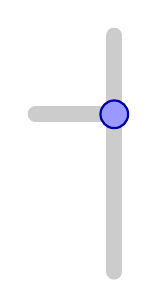
\begin{tikzpicture}
  \draw [line width=2mm, color=white!60!gray, line cap=round] (1, 0) to (1, 3);

  \draw [line width=2mm, color=white!60!gray, line cap=round] (0, 2) to (1, 2);

  \filldraw[thick, fill=white!60!blue, draw=black!30!blue] (1, 2) circle (5pt);
\end{tikzpicture}
\end{multicols}

\newpage

\subsection{Elementi}
Na zemljevid lahko dodamo ostale elemente mest, kot so reke, jezera, parke, polja.
Mesta pa lahko vsebujejo tudi točkovne elemente, kot so drevesa, križišča, restavracije.

\begin{CITY}
  river "NAME" {
    @\Var{COMMANDS}@
  }

  lake "NAME" {
    @\Var{COMMANDS}@
  }

  park "NAME" {
    @\Var{COMMANDS}@
  }

  field {
    @\Var{COMMANDS}@
  }

  tree @\Var{POINT}@

  junction @\Var{POINT}@

  restaurant "NAME" @\Var{POINT}@
\end{CITY}

\subsection{Ukazi}
Poleg osnovnih ukazov za izris lahko dodamo še druge: ukaz za izris elipse, dele krožnic, črte in krivulje sestavljene iz več segmentov (to je eden od načinov da se izognemo podvajanju točk), lahko definiramo razširjen ukaz \Fun{bend}, kjer se kota na vsaki strani razlikujeta, dodamo lahko parameter, ki nam pove kako ohlapna naj bo krivulja, lahko pa dodamo tudi ukaz \Fun{curve}, ki nam omogoča da prosto izberemo kontrolne točke Bezierjeve krivulje.

\begin{CITY}
  ellip(@\Var{POINT}@, @\Var{AXIS}@, @\Var{AXIS}@)

  arc(@\Var{POINT}@, @\Var{ANGLE}@, @\Var{ANGLE}@)

  polyline(@\Var{POINTS}@)

  polyspline(@\Var{POINTS}@)

  bend(@\Var{POINT}@, @\Var{POINT}@, @\Var{ANGLE}@, @\Var{ANGLE}@)

  bend(@\Var{POINT}@, @\Var{POINT}@, @\Var{ANGLE}@, @\Var{ANGLE}@, @\Var{LOOSENESS}@)

  curve(@\Var{POINT}@, @\Var{POINT}@, @\Var{CONTROL}@)

  curve(@\Var{POINT}@, @\Var{POINT}@, @\Var{CONTROL}@, @\Var{CONTROL}@)
\end{CITY}

\subsection{Konstrukti}

\subsubsection{Konstante in spremenjljivke}
Konstrukt \Keyword{let} omogoča, da ustvarite novo konstanto.
Tako boste lahko določene točke shranili in jih nato večkrat uporabili.
Predlagamo, da uporabite dinamično in strogo tipiziranje.
Po želji lahko dodate tudi spremenljivke.

\begin{CITY}
  road "Oljcna pot" {
    let p = (@\Num{2}@, @\Num{2}@);
    let q = (@\Num{5}@, @\Num{4}@);

    bend((@\Num{1}@, @\Num{1}@), p, @\Num{20}@);
    bend(p, (@\Num{3}@, @\Num{1}@), @\Num{40}@);
    line(p, (@\Num{2}@, @\Num{5}@));
    bend((@\Num{2}@, @\Num{3}@), q, @\Num{20}@);
    line(q, (@\Num{6}@, @\Num{4}@))
  }
\end{CITY}

\subsubsection{Matematični izrazi}
Pogosto je koristno, da lahko izračunamo novo lokacijo na podlagi parametrov ali obstoječih lokacij.
Da boste lahko dobili elemente točk je potrebno vgraditi funkciji \Fun{fst} in \Fun{snd}, ki vrneta prvi in drugi element točke.

\begin{CITY}
  road "Oljcna pot" {
    let bound = @\Num{1}@;
    let s = (bound, bound);
    let p = (fst(s) + @\Num{1}@, snd(s) + @\Num{1}@);
    let q = (@\Num{5}@, @\Num{4}@);

    bend(s, p, @\Num{20}@);
    bend(p, (@\Num{3}@, @bound@), @\Num{40}@);
    line(p, (@\Num{2}@, @\Num{5}@));
    bend((@\Num{2}@, @\Num{3}@), q, @\Num{20}@);
    line(q, (@\Num{6}@, @\Num{4}@))
  }
\end{CITY}

\subsubsection{Kontrola toka}

\begin{CITY}
  building "Hotel Fiesa" {
    if n > @\Num{1}@ {
      line((@\Num{1}@, @\Num{1}@), (@\Num{2}@, @\Num{2}@))
    } else {
      line((@\Num{2}@, @\Num{1}@), (@\Num{1}@, @\Num{2}@))
    }

    for i = @\Num{1}@ to @\Num{3}@ {
      box((@\Num{1}@, i), (@\Num{2}@, i + @\Num{1}@))
    }
  }
\end{CITY}

\subsubsection{Abstrakcija}
Določene kompleksne elemente lahko ponovimo na poljubnih mestih, tako da dodamo procedure \Keyword{procedure} in funkcije \Keyword{lambda}.
Poleg tega, pa lahko uporabimo ta konstrukta za poljubne izračune, kar še dodatno dvigne izraznost jezika.
Za rekurzivne funkcije lahko dodamo konstrukt $\Keyword{rec let}$.
Če so spremenljivke dinamično tipizirane pa lahko rekurzijo podpremo tudi brez dodatnih konstruktov, tako da definiramo operator, ki nam vrne fiksno točko \Fun{fix} \footnote{https://en.wikipedia.org/wiki/Fixed-point\_combinator}.
Predstavljene procedure in funkcije vrnejo zadnjo vrednost, lahko pa definiramo tudi ukaz \Keyword{return}, ki ga lahko uporabimo tudi za predčasen zaključek izvajanja.

\begin{CITY}
  procedure row(p) {
    for i = @\Num{1}@ to @\Num{3}@ {
      box((fst(p), snd(p) + i), (fst(p) + @\Num{1}@, snd(p) + i + @\Num{1}@))
    }
  };

  building "Hotel Fiesa" {
    let square = lambda(x) {x * x};
    row((@\Num{1}@, square(@\Num{2}@)))
  }
\end{CITY}

\subsubsection{Seznami}
Koordinate lahko služijo tudi kot pari.
Z uporabo parov je mogoče enostavno podpreti enojno povezane sezname.
Za rep para lahko uporabimo enoto \Keyword{nil}.
Podpremo lahko tudi zanko \Keyword{foreach}, ki se izvede za vsak element seznama.
Prav tako pa lahko definiramo tudi lepšo sintakso, ki se pretvori v predstavitev s pari.

\begin{CITY}
  building "Hotel Fiesa" {
    let list = (@\Num{1}@, (@\Num{2}@, (@\Num{3}@, nil)));

    foreach x in list {
      box((@\Num{1}@, x), (@\Num{2}@, x + @\Num{1}@))
    };

    let fancy = [@\Num{1}@, @\Num{2}@, @\Num{3}@]
  }
\end{CITY}

\subsubsection{Operacije nad poligoni}
Implementiramo lahko operacije nad poligoni, unijo, presek, razliko.
Za implementacijo razike moramo podpreti tudi poligone z luknjami.

\subsubsection{Tansformacije}
Dodamo lahko tudi transformacije referenčnega okvirja.
Na primer, lahko premaknemo izhodišče in nato lokacije sledečih konstruktov opišemo relativno glede na premaknjeno izhodišče.

\begin{CITY}
  city "Positions" {
    translate (@\Num{5}@, @\Num{3}@);
    marker (@\Num{0}@, @\Num{0}@)
  }
\end{CITY}

\subsection{Sintaktični sladkor}
Poleg (ali namesto) ukazov lahko uporabimo tudi bolj strnjeno in elegantno sintakso.
Tukaj namesto ukaza \Fun{line} uporabljamo operator, prav tako pa združimo dele ceste, ki se držijo skupaj (tako se lahko izognemo podvajanju točk).
Sintaktični sladkor lahko dodate kjerkoli se vam zdi smiselno.

\begin{CITY}
  road "Oljcna pot" {
    (@\Num{1}@, @\Num{1}@) -- bend @\Num{20}@ (@\Num{2}@, @\Num{2}@) -- bend @\Num{40}@ (@\Num{3}@, @\Num{1}@);
    (@\Num{2}@, @\Num{2}@) -- (@\Num{2}@, @\Num{5}@);
    (@\Num{2}@, @\Num{3}@) -- bend @\Num{20}@ (@\Num{5}@, @\Num{4}@) -- (@\Num{6}@, @\Num{4}@);
  }
\end{CITY}

\subsection{3D}
Poleg longitude in latitude lahko dodamo točkam še nadmorsko višino ali višino stavbe.
V primeru, da boste izdelali 3D izrisovalnik lahko za izris uporabite tudi te informacije.

\subsection{Povpraševanja}
Dodate lahko povpraševanja nad modelom, torej lahko poiščemo elemente znotraj regije zanimanja.
Na primer, če imamo podano trenutno lokacijo lahko poiščemo restavracije, ki so v bližini.
Povpraševanja so lahko del jezika za opis infrastrukture ali samostojen jezik.
Tudi tukaj lahko za pohitritev iskanja uporabimo R-drevo.

\begin{multicols}{2}
\begin{CITY}
  city "Restaurants" {
    marker (@\Num{0}@, @\Num{0}@);
    marker (@\Num{1}@, @\Num{1}@);
    marker (@\Num{3}@, @\Num{2}@);
    marker (@\Num{7}@, @\Num{3}@);
    marker (@\Num{4}@, @\Num{6}@);
    marker (@\Num{5}@, @\Num{3}@);
    marker (@\Num{3}@, @\Num{5}@);

    let roi = (@\Num{3}@, @\Num{4}@);
    foreach x in neigh(roi, 3) {
      highlight x
    }
  }
\end{CITY}

\columnbreak

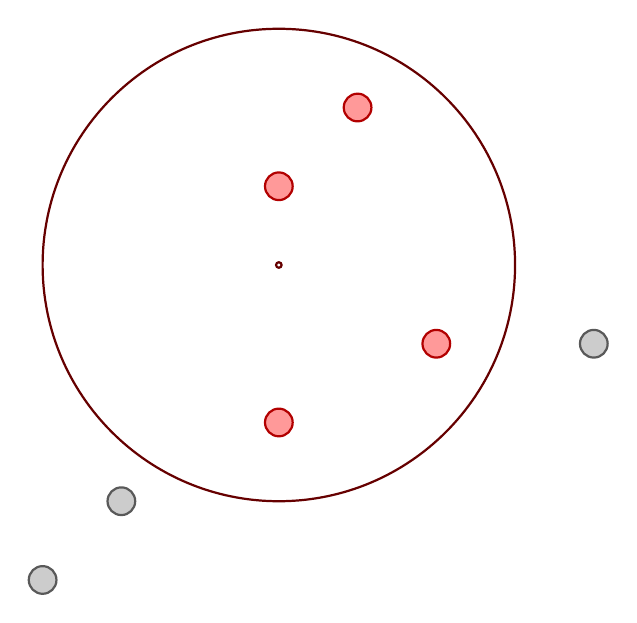
\begin{tikzpicture}
  \filldraw[thick, fill=white!60!gray, draw=black!30!gray] (0, 0) circle (5pt);
  \filldraw[thick, fill=white!60!gray, draw=black!30!gray] (1, 1) circle (5pt);
  \filldraw[thick, fill=white!60!red, draw=black!30!red] (3, 2) circle (5pt);
  \filldraw[thick, fill=white!60!gray, draw=black!30!gray] (7, 3) circle (5pt);
  \filldraw[thick, fill=white!60!red, draw=black!30!red] (4, 6) circle (5pt);
  \filldraw[thick, fill=white!60!red, draw=black!30!red] (5, 3) circle (5pt);
  \filldraw[thick, fill=white!60!red, draw=black!30!red] (3, 5) circle (5pt);
  \draw[thick, draw=black!60!red] (3, 4) circle (3);
  \draw[thick, draw=black!60!red] (3, 4) circle (1pt);
\end{tikzpicture}
\end{multicols}

\subsection{Meta podatki}
Vsakemu elementu v mestu lahko dodamo poljubne meta podatke.
Te metapodatke lahko kasneje uporabimo tudi za obogatitev izrisa.

\begin{CITY}
  city "Monitoring stations" {
    marker "Edvard Rusjan" (@\Num{8}@, @\Num{3}@) {
      set("precipitation", @\Num{0.93}@);
    }
  }
\end{CITY}

\subsection{Povezani podatki}
Metapodatke lahko pridobimo direktno iz zunanjih virov.
Na primer, tako podatke o infrastrukturi direktno povežemo z podatki iz merilnih postaj.

\begin{CITY}
  let data = link("https://www.monitoring-station.com/json");

  city "Monitoring stations" {
    marker "Edvard Rusjan" (@\Num{8}@, @\Num{3}@) {
      set("precipitation", data["Edvard Rusjan"].precipitation)
    }
  }
\end{CITY}

\subsection{Časovno odvisni podatki}
Elemenom lahko dodamo tudi čas nastanka, tako lahko opišemo spremembe v infrasktrukturi skozi neko časovno obdobje.

\subsection{Dostop do stanja izrisovalnika}

Jeziku lahko dodamo dostop do stanja izrisovalnika.
Dodamo lahko pretekel čas, kar nam omogoča opis animacij.
Dodamo lahko trenutno pozicjo miške, torej lahko določimo regijo zanimanja z miško.
Dodamo lahko vgrajene funkcije, torej lahko znotraj jezika izvedemo kompleksne operacije, ki so implementirane v sklopu izrisovalnika.


\end{document}
